\documentclass[../main.tex]{subfiles}

\begin{document}


\practica{Comunicación remota con \emph{ThingsBoard}}

    \subsection{Objetivos}
        \begin{itemize}
            \item Entender y configurar la plataforma de \emph{ThingsBoard}.
            \item Programar el STM32F723 para comunicarse con \emph{ThingsBoard}, enviando y recibiendo datos.
            \item Entender los protocolos de comunicación como MQTT.
        \end{itemize}

    \subsection{Fundamentos teóricos}
        
        En general, cualquier plataforma empotrada hoy en día tiene cierta conectividad con la red. Desde electrodomésticos inteligentes hasta estaciones de monitorización atmosférica, pasando por bombillas que pueden cambiarse de color desde el móvil, todos estos dispositivos pueden enviar y recibir información desde internet.

        Para ello existen numerosos protocolos. Uno de los más extendidos, por su ligereza y versatilidad, es \textbf{MQTT}. \textbf{MQTT} es un protocolo ligero para el intercambio de mensajes, diseñado para la comunicación en redes con ancho de banda limitado, y por dispositivos con capacidad de computación reducida. Debido a su simplicidad y escalabilidad, MQTT es de particular interés para aplicaciones de Internet de las cosas (IoT).

        MQTT utiliza un formato de mensaje binario (\Cref{fig:mqtt_packet}), que reduce enormemente la cantidad de información transmitida frente a otros protocolos basados en texto como \textbf{HTTP}.

        \begin{figure}[h]
            \centering
            \begin{tikzpicture}[
                font=\sffamily,
                box/.style={draw, rectangle, minimum height=1.1cm, align=center, inner sep=6pt, line width=0.8pt},
                fh/.style={box, fill=blue!15, draw=blue!70!black},
                vh/.style={box, fill=green!15, draw=green!70!black},
                pl/.style={box, fill=orange!15, draw=orange!70!black},
                subbox/.style={box, fill=blue!5, draw=blue!40!black, font=\sffamily\small}
            ]

                % Level 1: Top-level Structure
                \node[fh, minimum width=4.5cm] (fixed) {\textbf{Fixed Header}\\(2 to 5 Bytes)};
                \node[vh, minimum width=3.5cm, right=0cm of fixed] (var) {\textbf{Variable Header}\\(Optional)};
                \node[pl, minimum width=4.0cm, right=0cm of var] (payload) {\textbf{Payload}\\(Optional)};

                \node[above=0.2cm of fixed.north west, anchor=south west, font=\sffamily\bfseries] {MQTT Control Packet Hierarchy};

                % Level 2: Fixed Header Breakdown
                \node[subbox, minimum width=6cm, anchor=north west] (byte1) at ($(fixed.south west) + (0,-1.2)$) {\textbf{Byte 1}\\Control Type \& Flags};
                \node[subbox, minimum width=6cm, right=0cm of byte1] (byte2) {\textbf{Byte 2\dots Byte 5}\\Remaining Length (1--4 Bytes)};

                \draw[thick, ->, >=stealth, blue!70!black] (fixed.south west) -- (byte1.north west);
                \draw[thick, ->, >=stealth, blue!70!black] (fixed.south east) -- (byte2.north east);

                % Level 3: Byte 1 Bit Breakdown
                \node[subbox, fill=blue!25, minimum width=3cm, anchor=north west] (type) at ($(byte1.south west) + (0,-1.2)$) {\textbf{Bits 7--4}\\Packet Type (15 types)\\e.g., $0001_2$ = CONNECT};
                \node[subbox, fill=blue!10, minimum width=3cm, right=0cm of type] (flags) {\textbf{Bits 3--0}\\Flags Specific to Type\\e.g., DUP, QoS, RETAIN};

                \draw[thick, ->, >=stealth, blue!70!black] (byte1.south west) -- (type.north west);
                \draw[thick, ->, >=stealth, blue!70!black] (byte1.south east) -- (flags.north east);

            \end{tikzpicture}
            \caption{Formato de los paquetes \textbf{MQTT}}
            \label{fig:mqtt_packet}
        \end{figure}

        En \textbf{MQTT} se distinguen los \emph{clientes} y los \emph{brokers}. Un cliente puede enviar mensajes al broker (conteniendo generalmente actualizaciones de valores etiquetados), y el broker reenvía estas actualizaciones a otros clientes que estén suscritos a dichos valores etiquetados. Las etiquetas se indican categorizadas, con cada categoría separada por ``/''. Así, se permiten suscripciones a categorías completas, por ejemplo (luego lo veremos en más detalle al hacer la práctica). Un ejemplo sencillo de esta estructura puede verse en \Cref{fig:mqtt_diagram}


        \begin{figure}[h]
            \centering
            \begin{tikzpicture}[
                font=\sffamily,
                % Define node styles
                node_base/.style={draw, thick, rectangle, rounded corners, minimum height=1.5cm, align=center, inner sep=10pt},
                broker/.style={node_base, fill=blue!10, draw=blue!70!black, minimum width=3cm, font=\sffamily\bfseries},
                client/.style={node_base, fill=white, draw=gray, minimum width=2.5cm},
                % Define arrow styles
                arrow_style/.style={-{Stealth[scale=1.0]}, thick},
                pub_arrow/.style={arrow_style, draw=red!70!black, densely dashed},
                sub_arrow/.style={arrow_style, draw=green!60!black}
            ]

                % --- 1. The MQTT Broker (The Core) ---
                \node[broker] (broker) {
                    \textbf{MQTT Broker} \\
                    (e.g., ThingsBoard) 
                };

                % --- 2. Client that is ONLY a Publisher (Sensor) ---
                \node[client, left=2.8cm of broker] (sensor) {
                    Temp. Sensor \\ (Kitchen) \\
                    \textbf{\textcolor{red!70!black}{Publisher}}
                };

                % --- 3. Client that is ONLY a Subscriber (Actuator) ---
                \node[client, right=2.5cm of broker] (lock) {
                    Front Door Lock \\
                    \textbf{\textcolor{green!60!black}{Subscriber}}
                };

                % --- 4. Client that is BOTH (The Hub) ---
                \node[client, above=2cm of broker] (hub) {
                    Smart Home Hub (Tablet) \\
                    \textbf{\textcolor{red!70!black}{Publisher}} \& \textbf{\textcolor{green!60!black}{Subscriber}}
                };


                % --- DRAWING INTERACTIONS AND FLOWS ---

                % Flow Set A: Temperature Data (Sensor -> Broker -> Hub)
                % Publish connection from sensor to broker
                \draw[pub_arrow] (sensor.east) -- (broker.west) 
                    node[midway, above, text=red!70!black, font=\small\bfseries] {PUBLISH}
                    node[midway, below, font=\footnotesize] {\texttt{home/kitchen/temp}}
                    node[midway, below=0.4cm, font=\footnotesize, fill=white] {Payload: \texttt{22.5°C}};

                % Subscribe connection from broker to hub
                \draw[sub_arrow] (broker.north) .. controls +(0,1.2) and +(0,-1.2) .. (hub.south)
                    node[midway, right=0.3cm, text=green!60!black, font=\small\bfseries, anchor=west] {SUBSCRIBE}
                    node[midway, right=0.3cm, font=\footnotesize, anchor=west, yshift=-0.4cm] {\texttt{home/kitchen/temp}};

                    
                % Flow Set B: Lock Command (Hub -> Broker -> Lock)
                % Publish connection from hub back to broker
                % Note: Using slightly different anchors to keep lines separated
                \draw[pub_arrow] ($(hub.south)+(-0.3,0)$) .. controls +(-0.8,-1.2) and +(-0.8,1.2) .. ($(broker.north)+(-0.3,0)$)
                    node[pos=0.3, left=0.1cm, text=red!70!black, font=\small\bfseries, anchor=east] {PUBLISH}
                    node[pos=0.3, left=0.1cm, font=\footnotesize, anchor=east, yshift=-0.4cm] {\texttt{home/door/lock}}
                    node[pos=0.3, left=0.1cm, font=\footnotesize, anchor=east, yshift=-0.7cm] {Payload: \texttt{UNLOCK}};

                % Subscribe connection from broker to lock
                \draw[sub_arrow] (broker.east) -- (lock.west)
                    node[midway, above, text=green!60!black, font=\small\bfseries] {SUBSCRIBE}
                    node[midway, below, font=\footnotesize] {\texttt{home/door/lock}};


                % --- LEGEND ---
                \node[draw, thick, rounded corners, fill=white, inner sep=6pt, anchor=north, yshift=-1cm] (legend) at (broker.south) {
                    \begin{minipage}{5cm}
                    \small \textbf{Legend:} \\
                    \tikz \draw[pub_arrow] (0,0) -- (0.6,0); \textcolor{red!70!black}{ Publish Message (Out)} \\
                    \tikz \draw[sub_arrow] (0,0) -- (0.6,0); \textcolor{green!60!black}{ Subscribe Message (In)} \\
                    Note: Red/Green dotted lines represent MQTT control packets (not physical cables).
                    \end{minipage}
                };
            \end{tikzpicture}
            \caption{Generic MQTT diagram}
            \label{fig:mqtt_diagram}
        \end{figure}

        \subsubsection{El módulo Wifi ESP-01S}

            Nuestro procesador no tiene manera de realizar comunicación inalámbrica, por tanto se utiliza un módulo externo \texttt{ESP-01S} conectado al conector \texttt{CN14}. Este módulo permite, a través de una comunicación \PER{UART} desde el procesador \MCU, establecer una conexión WiFi y enviar o recibir datos a través de protocolos como \texttt{HTTP} y \texttt{TCP}, que serán vistos desde nuestra aplicación a través de la \PER{UART}. 

            Nosotros lo veremos solo como usarios y con un conjunto reducido de comandos. Puedes consultar la documentación completa en \url{https://espressif-docs.readthedocs-hosted.com/projects/esp-at/en/release-v2.2.0.0_esp8266/AT_Command_Set/index.html}.
        
    \subsection{Desarrollo de la práctica}

        Para realizar la práctica, vamos a hacer uso de un \emph{broker} llamado \textbf{ThingsBoard} (\url{https://thingsboard.io/}). Es una plataforma online que ofrece, de manera gratuita, un \emph{broker} para hasta 5 dispositivos. Como solo tenemos uno, será suficiente. 

        Para nuestro cliente, utilizaremos las librerías de Eclipse Paho MQTT (\url{https://github.com/eclipse-paho/paho.mqtt.embedded-c}), una implementación ligera de MQTT para dispositivos empotrados.
        
        \subsubsection{Creando cuenta y dispositivo en \emph{ThingsBoard}}

            Lo primero de todo es crear una cuenta gratuita en \emph{Thingsboard Cloud Europe} (\url{https://eu.thingsboard.cloud/signup}). Veremos algo similar a la \Cref{fig:thingsboard_startup} al iniciar.


            \begin{figure}
                \centering
                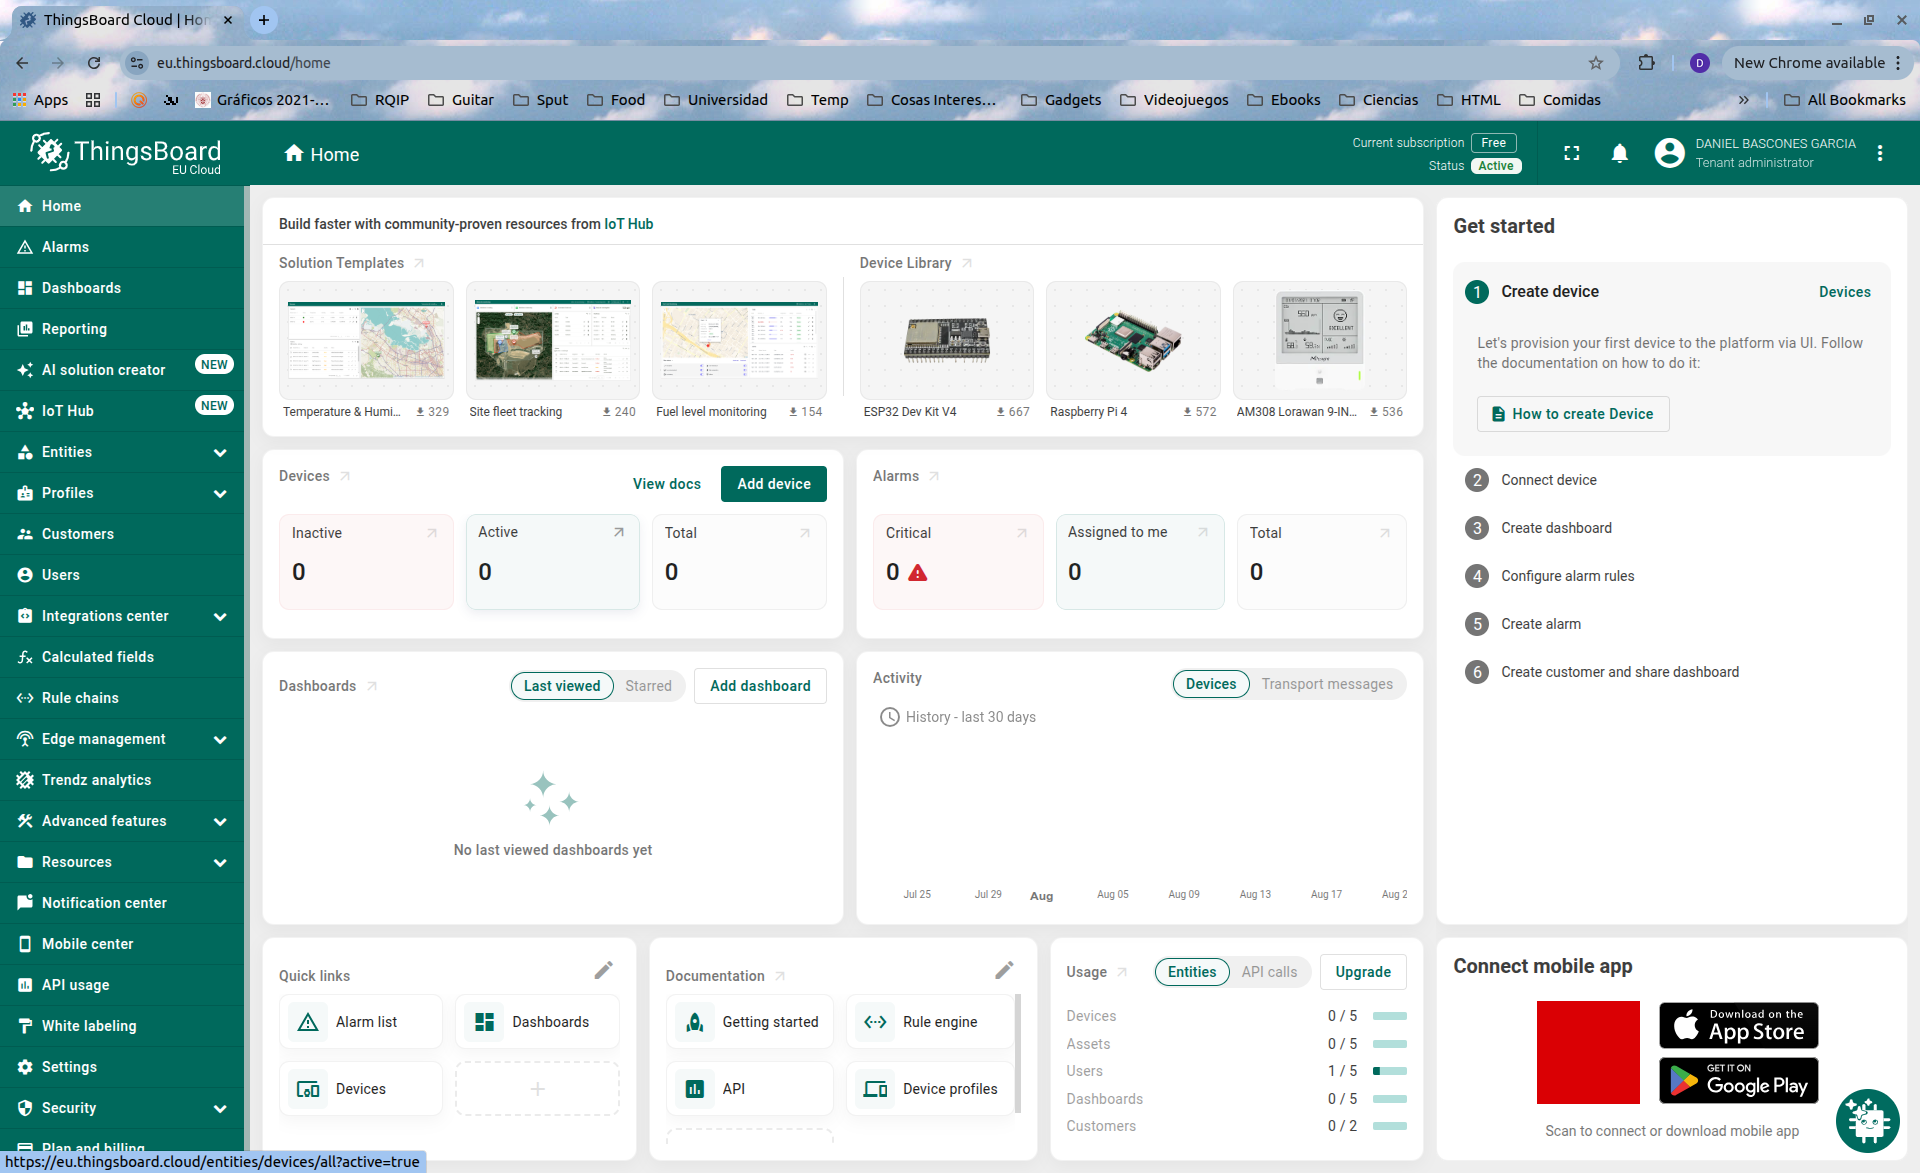
\includegraphics[width=\textwidth]{res/thingsboard_startup.png}
                \caption{Pantalla inicial de \emph{ThingsBoard} tras iniciar sesión}
                \label{fig:thingsboard_startup}
            \end{figure}

            A continuación, tendremos que crear un dispositivo (desde el panel ``Devices'') (que representará nuestra placa \BOARD) como en la \Cref{fig:thingsboard_add_device}.

            \begin{figure}
                \centering
                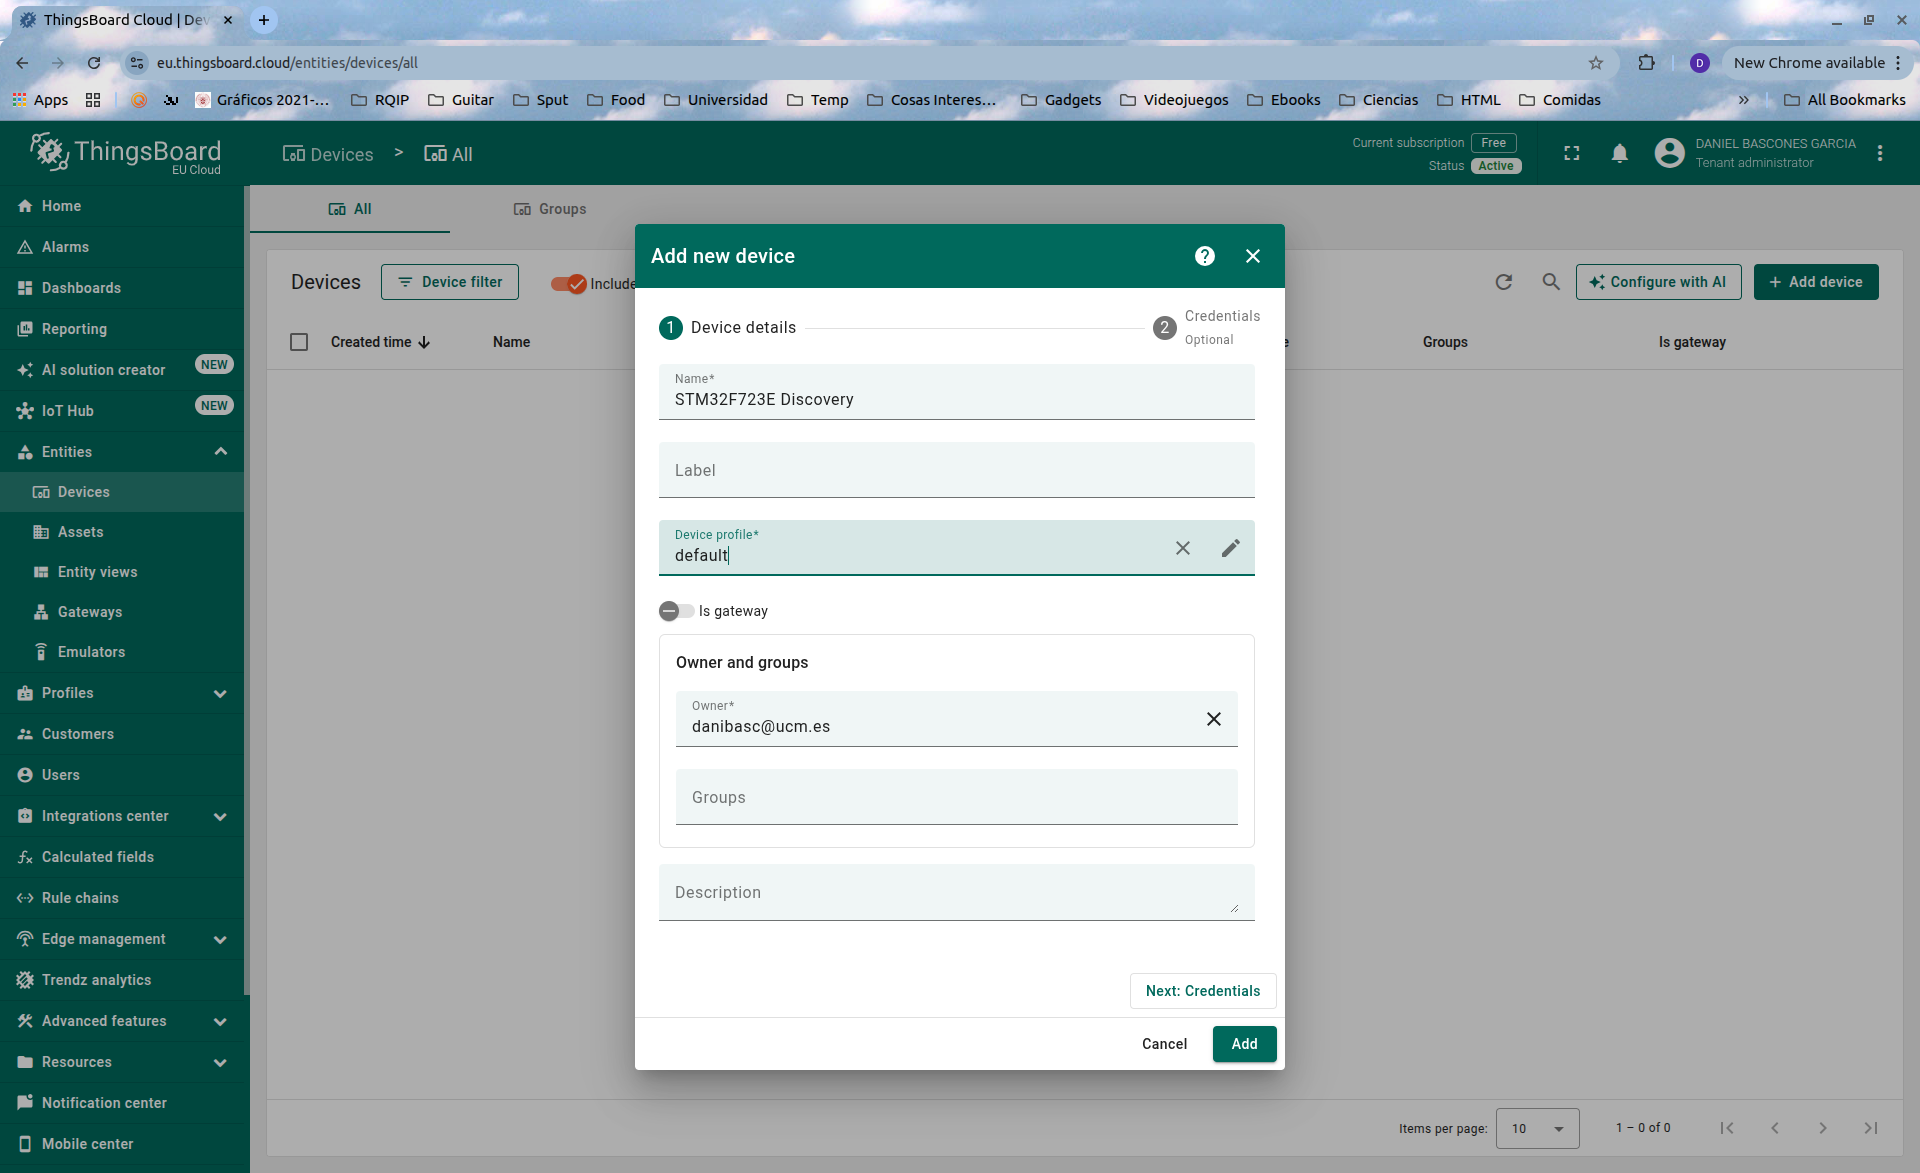
\includegraphics[width=\textwidth]{res/thingsboard_add_device.png}
                \caption{Pantalla de añadir un nuevo dispositivo}
                \label{fig:thingsboard_add_device}
            \end{figure}

            Para conectarnos posteriormente, necesitaremos identificarnos (y demostrar, desde el dispositivo, que tenemos derecho a enviar/recibir información). Aunque hay varias maneras de hacerlo, nosotros lo haremos con un \emph{token} de acceso. Para ello, entra en la configuración del dispositivo y busca el \emph{token} dentro de \emph{credentials} (\Cref{fig:thingsboard_credentials}). Anótalo bien, lo necesitarás.

            \begin{figure}
                \centering
                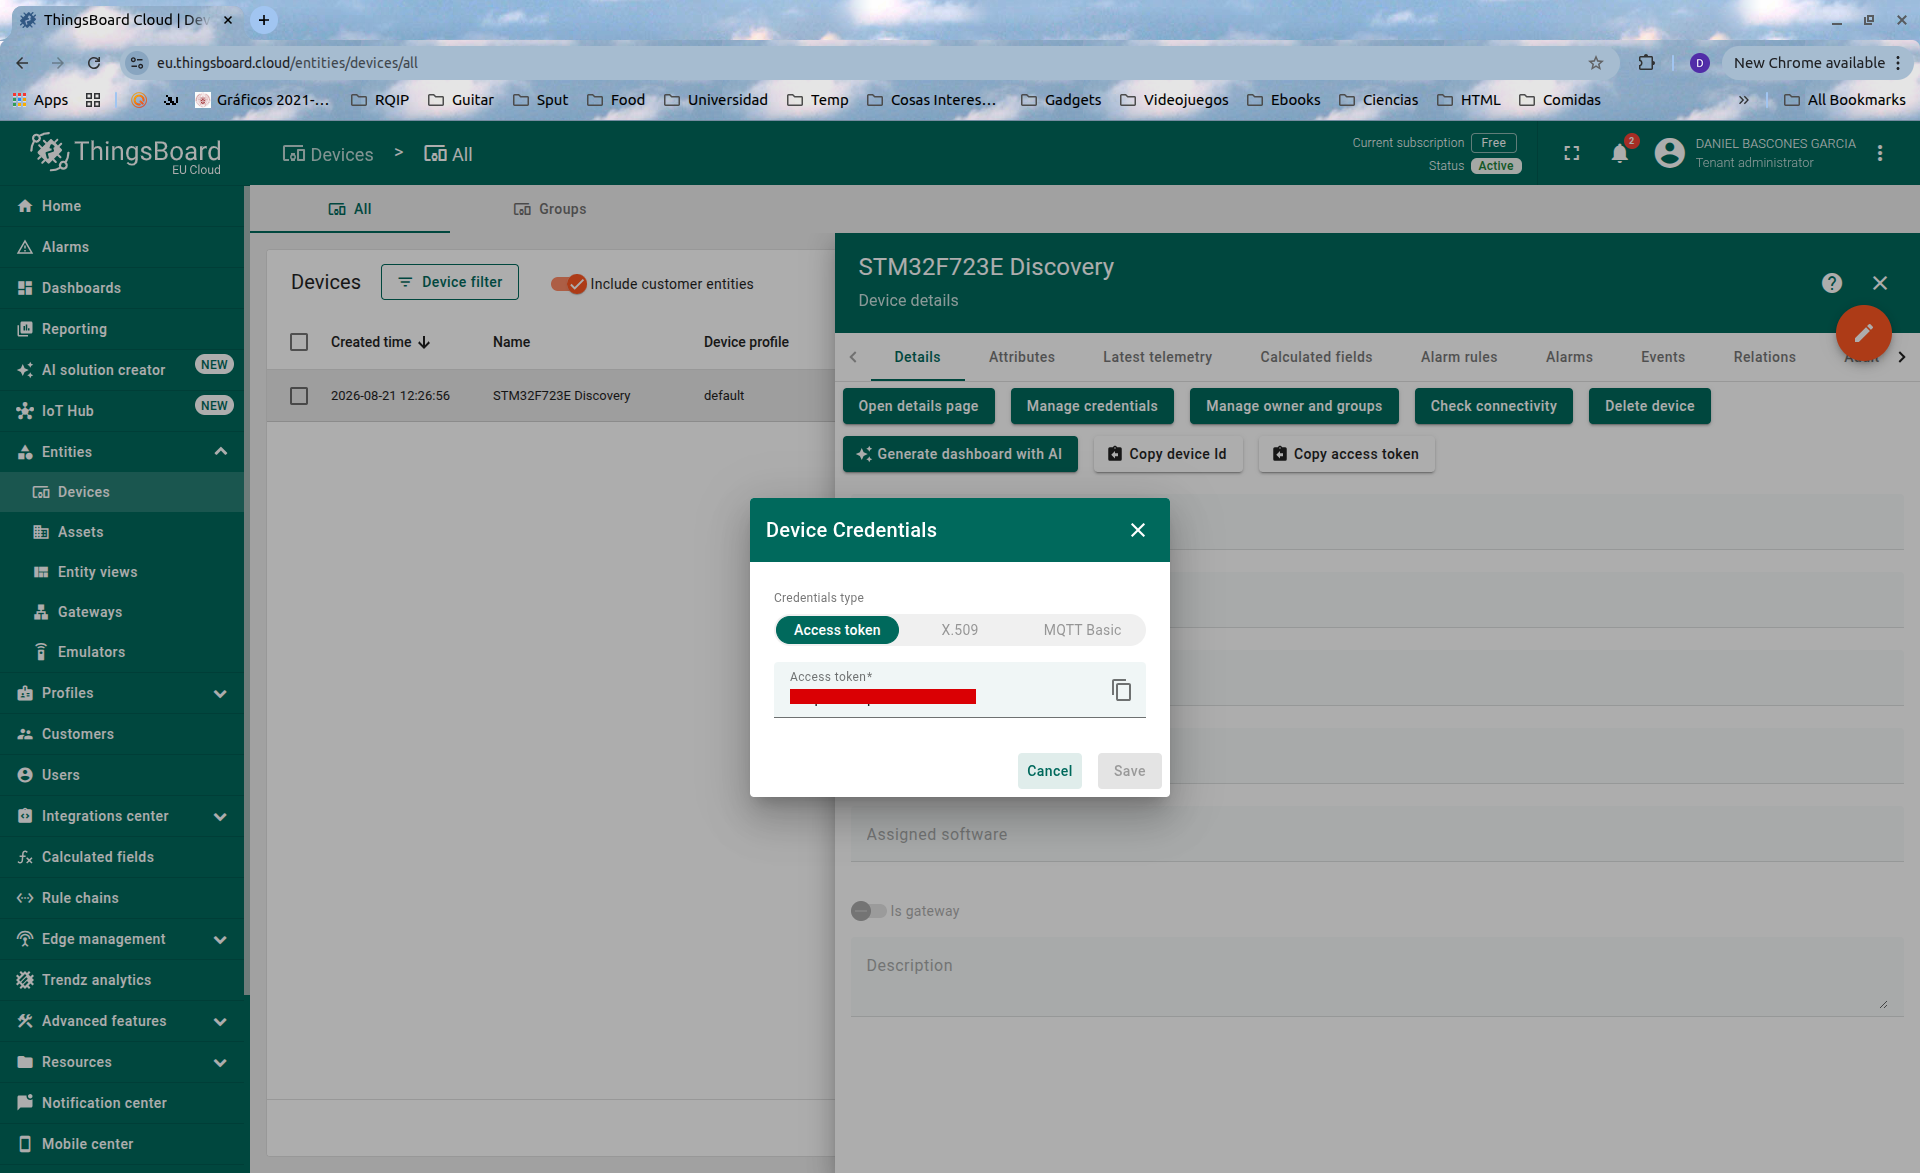
\includegraphics[width=\textwidth]{res/thingsboard_credentials.png}
                \caption{Credenciales de nuestro dispositivo}
                \label{fig:thingsboard_credentials}
            \end{figure}

        \subsubsection{Programando nuestro dispositivo para conectar}

            En esta práctica no vas a tener que programar demasiadas cosas, ya que la complejidad de las librerías es elevada. La base del código, ya funcional, está hecha, y tiene esta pinta:

            \dirtree{%
                .1 thingsboard\_data\_control/.
                .2 Src/\DTcomment{\textcolor{gray}{-- Source code directory}}.
                .3 main.c\DTcomment{\textcolor{gray}{-- Core application entry point}}.
                .2 Inc/\DTcomment{\textcolor{gray}{-- Include files}}.
                .3 bsp.c\DTcomment{\textcolor{gray}{-- Board Support Package Code}}.
                .3 bsp.h\DTcomment{\textcolor{gray}{-- Board Support Package Header}}.
                .3 ESP01S\_config\_template.h\DTcomment{\textcolor{gray}{-- Template to fill with config constants}}.
                .3 ESP01S.c\DTcomment{\textcolor{gray}{-- ESP01S Controller Code}}.
                .3 ESP01S.h\DTcomment{\textcolor{gray}{-- ESP01S Controller Header}}.
                .3 MQTT*\DTcomment{\textcolor{gray}{-- Eclipse Paho Embedded MQTT Library}}.
                .3 RingBuffer.c\DTcomment{\textcolor{gray}{-- Helper Receiver Buffer Code}}.
                .3 RingBuffer.h\DTcomment{\textcolor{gray}{-- Helper Receiver Buffer Header}}.
                .3 StackTrace.h\DTcomment{\textcolor{gray}{-- Eclipse Paho Embedded MQTT Library}}.
            }
    
            Lo único que falta es renombrar el archivo \texttt{ESP01S\_config\_template.h} por \texttt{ESP01S\_config.h}, y configurar las credenciales del punto WiFi a utilizar (puede ser vuestro teléfono en modo AP) y el \emph{token} que hemos obtenido anteriormente.

            Al lanzar ahora la aplicación, deberíamos ver por el terminal (recuerda abrirlo con \texttt{picocom}) los siguientes mensajes de depuración):

            \begin{lstlisting}
                [ESP] Testing ESP01S AT Communication...
                [ESP] Disabling Echo...
                [ESP] Setting Station Mode...
                [ESP] Disabling MUX (Single Conn Mode)...
                [ESP] Enabling Transparent Passthrough Mode...
                [ESP] Connecting to SSID: WIFI_SSID ..
                [MQTT] Connecting to eu.thingsboard.cloud:1883...
                [MQTT] Entering passthrough streaming...
                [MQTT RX] CONNACK 0x00: Connection Accepted!
                [MQTT RX] SUBACK Received! Granted QoS: 0
                [MQTT] Connected & Subscribed successfully!
                [SYSTEM] Ready! Streaming over MQTT...
                [MQTT TX] {"temp":20.50,"counter":1,"touch_x":15,"touch_y":20}
                [MQTT TX] {"temp":21.00,"counter":2,"touch_x":30,"touch_y":40}
                [MQTT TX] {"temp":21.50,"counter":3,"touch_x":45,"touch_y":60}
                [MQTT TX] {"temp":22.00,"counter":4,"touch_x":60,"touch_y":80}
                [MQTT TX] {"temp":22.50,"counter":5,"touch_x":75,"touch_y":100}
            \end{lstlisting}

            Con esto, hemos establecido la conexión al \emph{broker} de \textbf{MQTT} de \emph{ThingsBoard}. Algunas cosas a notar es que, debido a la simplicidad de esta implementación (si echas un vistazo al código, verás que se implementa un cliente ``a mano''), no tenemos control de errores ni QoS superior a 0. Es decir, que si algún mensaje se pierde, se ha perdido y no se recupera.

            De momento, en cualquier caso, estamos enviando mensajes al servidor con varias variables (en este caso, creadas de manera sintética). Si entramos en \emph{ThingsBoard}, dentro de la gestión del dispositivo, deberíamos ver ya las variables de telemetría como en la \Cref{fig:thingsboard_telemtry}.

            \begin{figure}
                \centering
                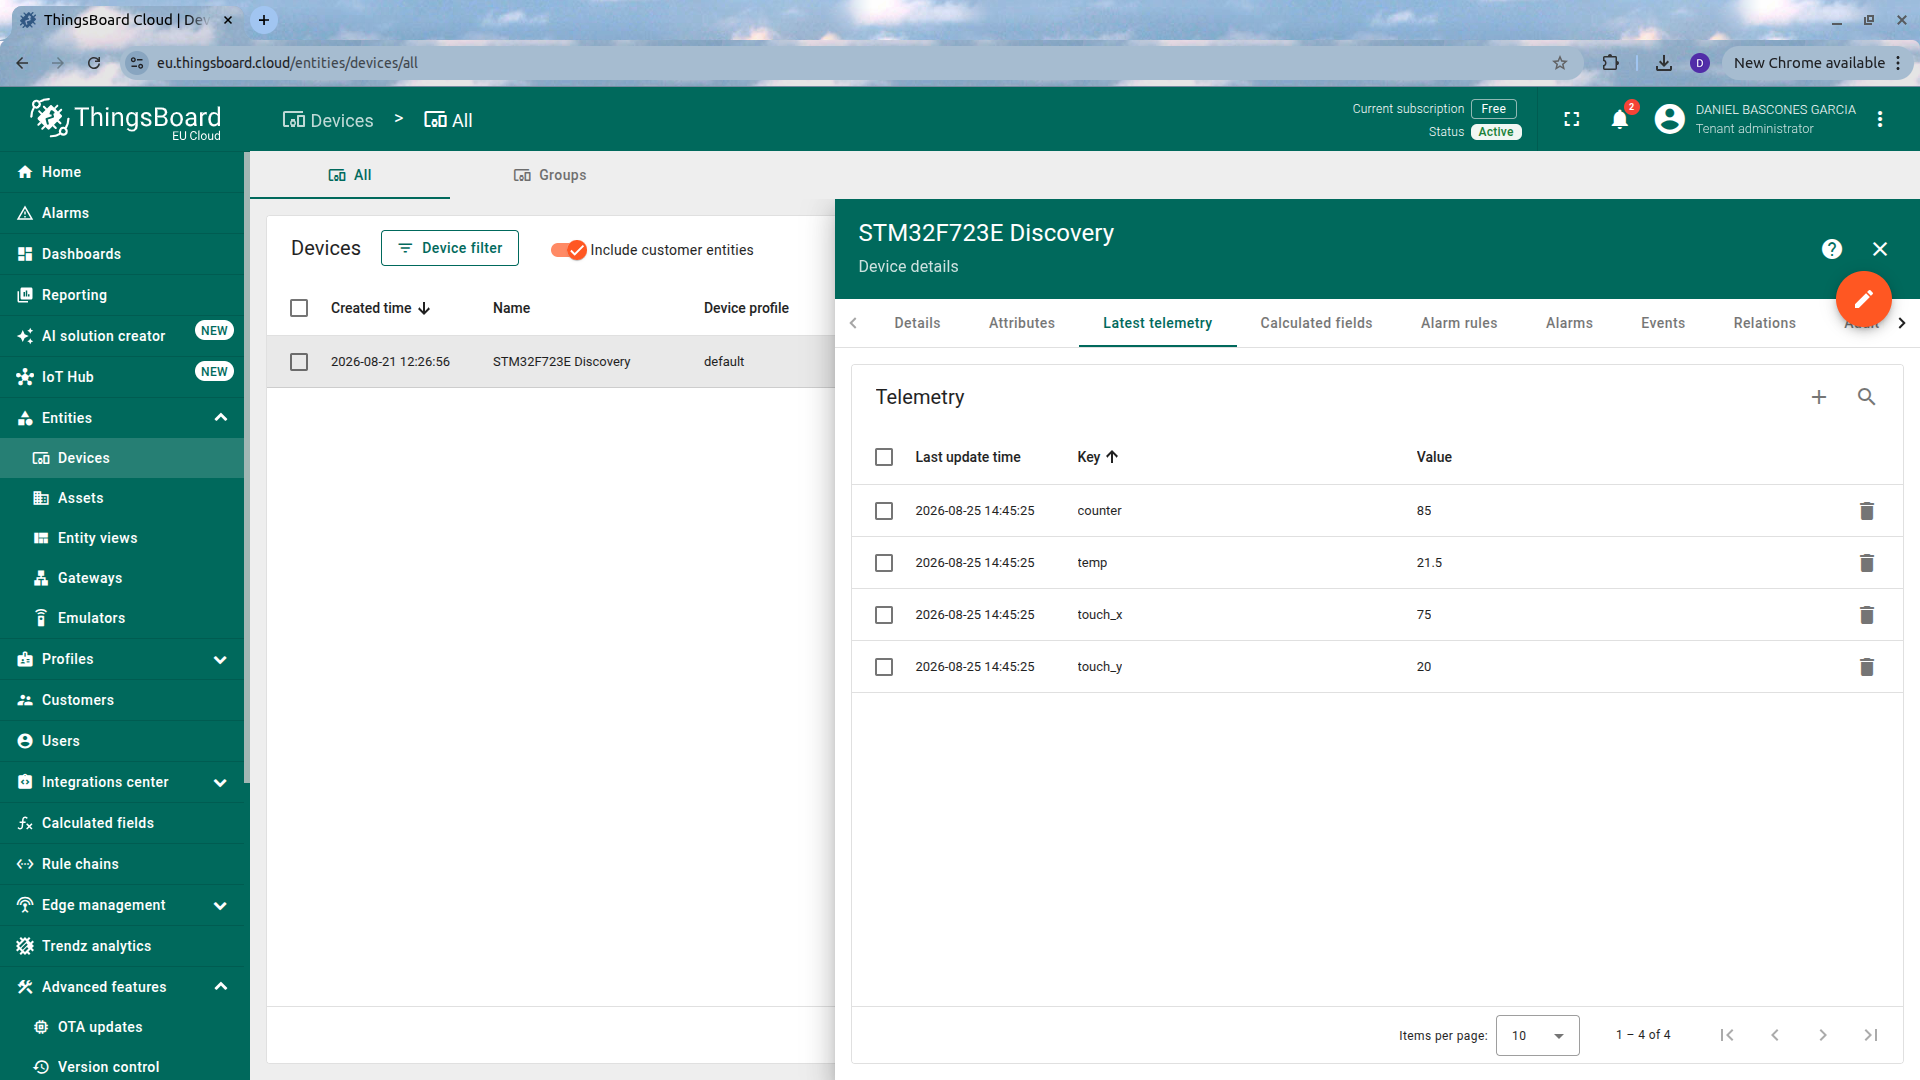
\includegraphics[width=\textwidth]{res/thingsboard_telemetry.png}
                \caption{Telemetría vista desde thingsboard}
                \label{fig:thingsboard_telemetry}
            \end{figure}

        \subsubsection{Visualización en \emph{ThingsBoard}}

            \emph{ThingsBoard} tiene un sistema de visualización muy potente para crear gráficas, así que vamos a aprovecharlo, para ver bien estos datos, en lugar de en una lista numérica. Lo primero para poder utilizarlo es crear un \emph{Dashboard} como en la \Cref{fig:thingsboard_dashboard}.

            \begin{figure}
                \centering
                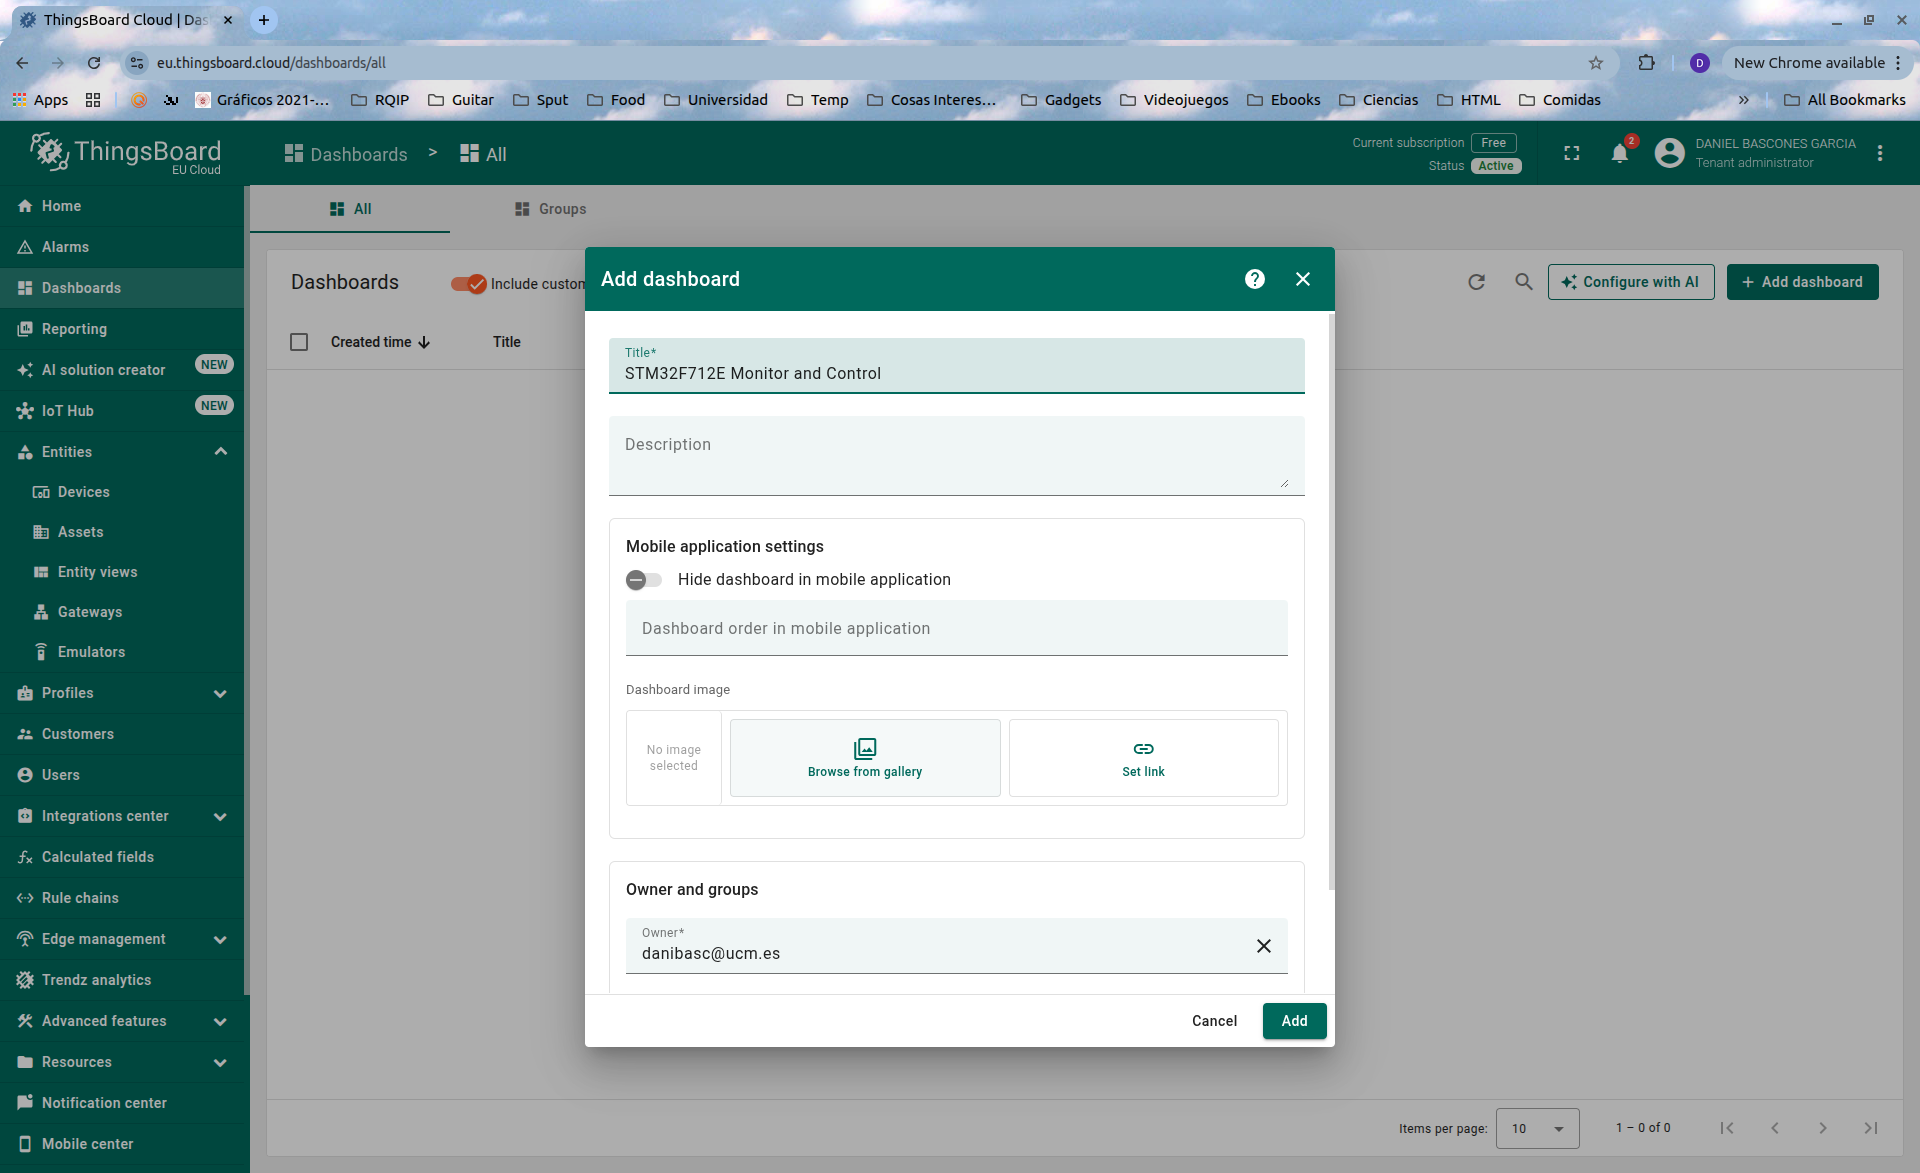
\includegraphics[width=\textwidth]{res/thingsboard_dashboard.png}
                \caption{Creación de un panel de control}
                \label{fig:thingsboard_dashboard}
            \end{figure}

            Ahora podemos añadir fácilmente elementos a nuestro panel desde el modo edición > añadir widget. Por ejemplo una gráfica que muestre la temperatura como en la \Cref{fig:thingsboard_temp_widget}. Asegúrate muy bien de que el nombre de la variable visualizada es el mismo que el que da nuestro dispositivo. A veces por defecto sale solo ``temp'' y no funcionará si es así. 

            \begin{figure}
                \centering
                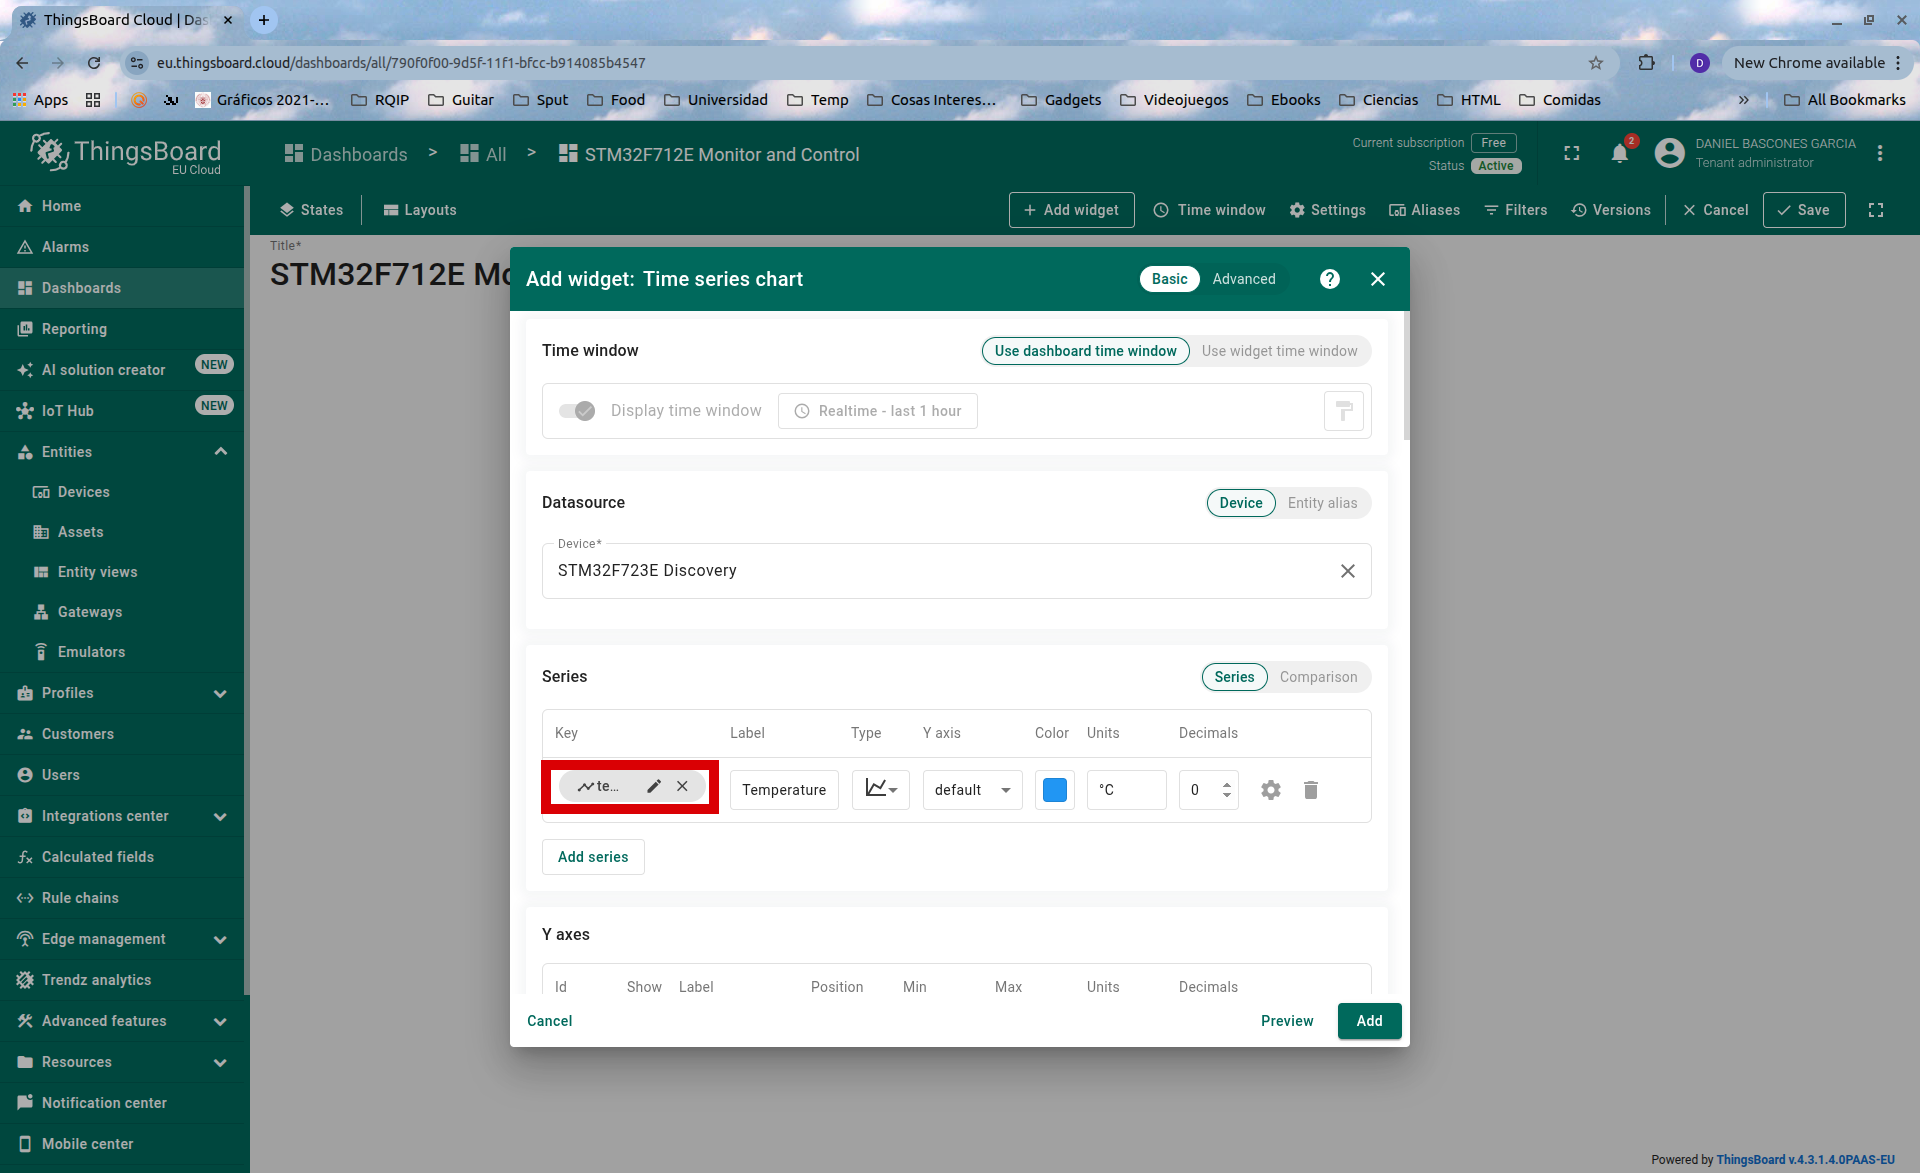
\includegraphics[width=\textwidth]{res/thingsboard_temp_widget.png}
                \caption{Añadiendo una gráfica que muestre la variable ``temperature''}
                \label{fig:thingsboard_temp_widget}
            \end{figure}

            También puedes añadir Widgets muy interesantes creados por la comunidad. Desde el mismo botón de Add Widget, pulsa en la pestaña de IoT Hub y busca ``scatter plot''. Puedes instalarlo desde ahí como muestra la \Cref{fig:thingsboard_install_widget}. Aprovecha para configurarlo mostrando \texttt{touch\_x} y \texttt{touch\_y}, las variables sintéticas que se están enviando.

            \begin{figure}
                \centering
                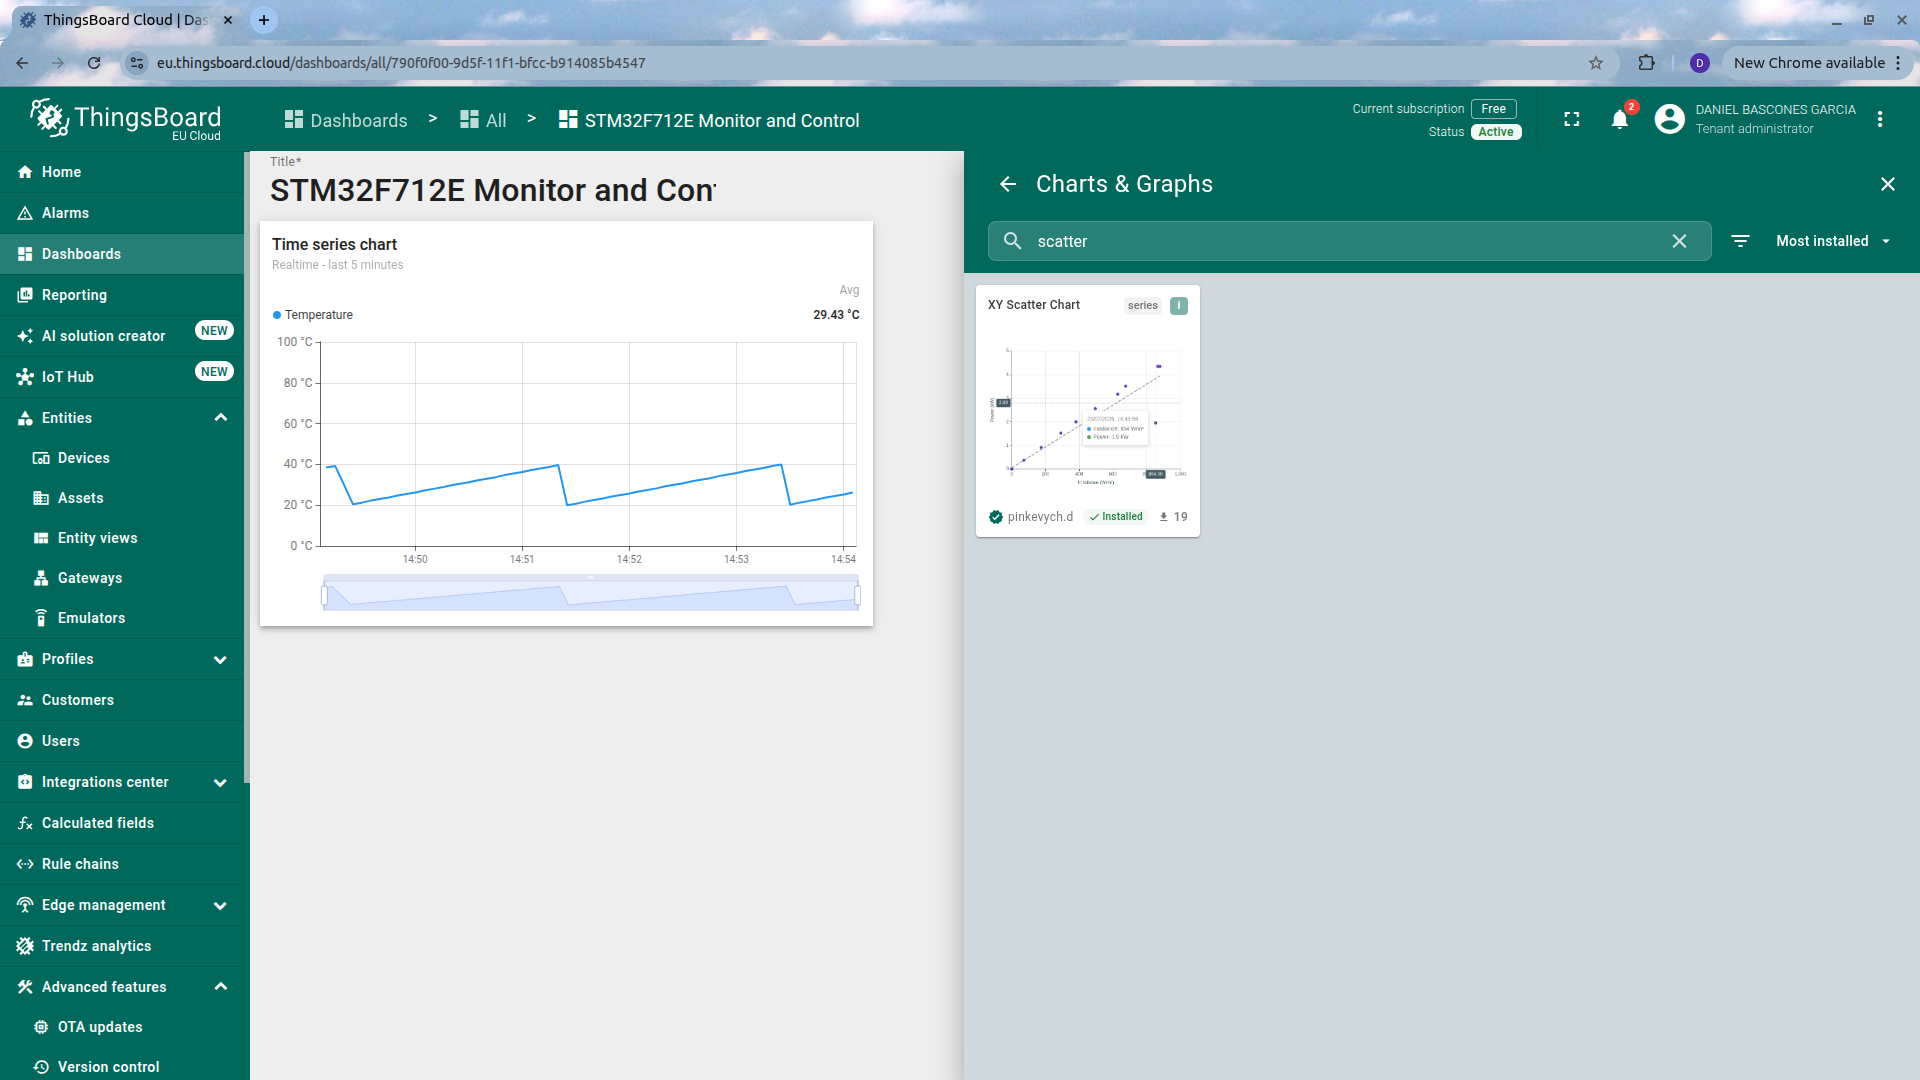
\includegraphics[width=\textwidth]{res/thingsboard_install_widget.png}
                \caption{Instalando nuevos widgets}
                \label{fig:thingsboard_install_widget}
            \end{figure}

            Tras haber añadido ambos widgets, deberías tener un panel similar a este, que se va actualizando automáticamente con los valores que llegan desde \BOARD.

            \begin{figure}
                \centering
                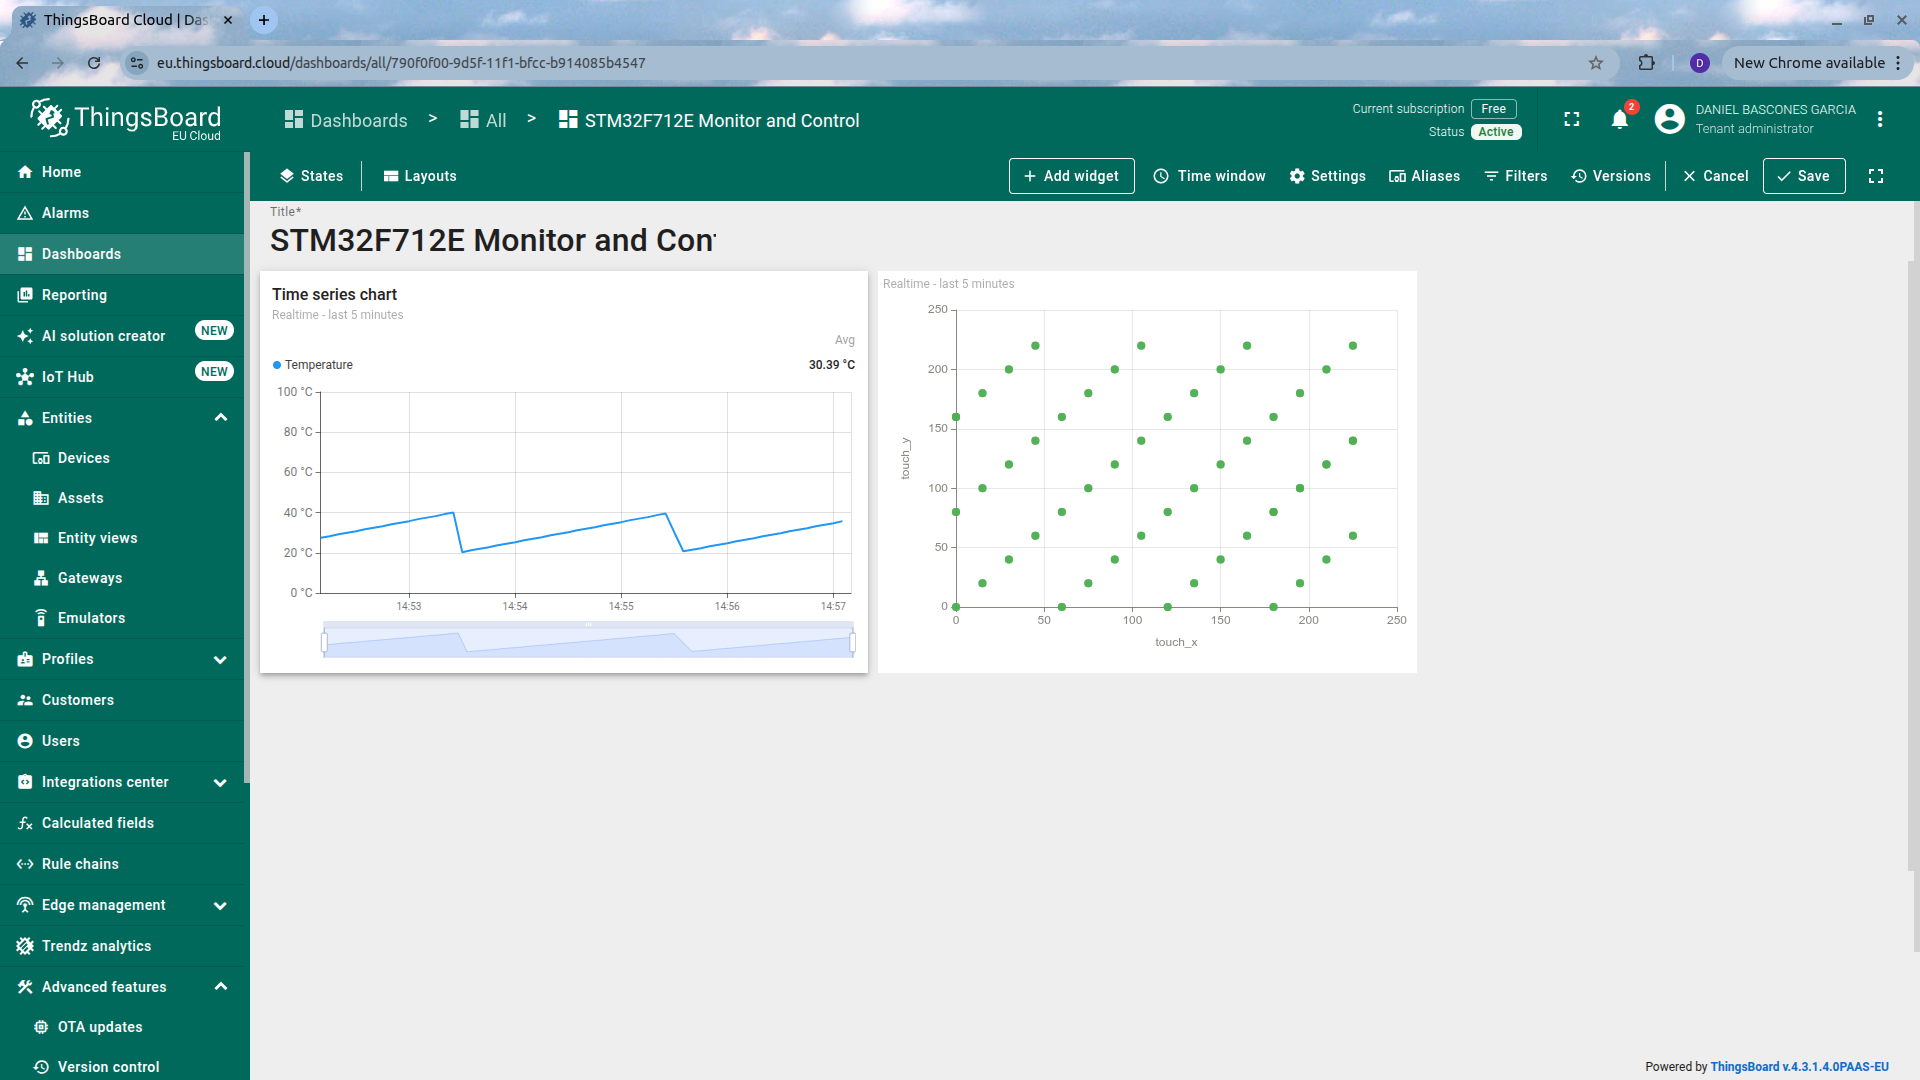
\includegraphics[width=\textwidth]{res/thingsboard_finished_dashboard.png}
                \caption{Panel finalizado}
                \label{fig:thingsboard_finished_dashboard}
            \end{figure}

            ¿Y... cómo se está haciendo toda esta magia detrás de las cámaras? Puedes analizar, viendo el código de \texttt{main.c} que cada cierto tiempo se llama a una función de envío de telemetría. Esta misma se reproduce a continuación:

            \begin{lstlisting}
                /*
                * Generic publish telemetry over MQTT
                */
                uint8_t ESP01S_SendTelemetry_MQTT(ESP01S_TypeDef * esp01s, float temp, uint32_t counter, uint16_t touch_x, uint16_t touch_y) {
                    uint8_t buf[256];
                    char payload[256];

                    int temp_int = (int)temp;
                    int temp_frac = (int)(abs((int)(temp * 100.0f)) % 100);

                    snprintf(payload, sizeof(payload),
                            "{\"temp\":%d.%02d,\"counter\":%lu,\"touch_x\":%u,\"touch_y\":%u}",
                            temp_int, temp_frac, (unsigned long)counter, touch_x, touch_y);

                    MQTTString topicString = MQTTString_initializer;
                    topicString.cstring = "v1/devices/me/telemetry";

                    int len = MQTTSerialize_publish(buf, sizeof(buf), 0, 0, 0, 0,
                                                    topicString, (unsigned char *)payload, strlen(payload));

                    UART_WriteBytes(esp01s->UARTx, buf, len);
                    Debug_Printf("[MQTT TX] %s\r\n", payload);
                    return 1;
                }
            \end{lstlisting}

            Puedes ver que primero se construye el \emph{payload MQTT} o carga, con las variables a enviar. A continuación, se declara el \emph{topic MQTT} o identificador donde enviar estas variables (por ejemplo, donde otros clientes podrían estar suscritos para escuchar cambios). El mensaje se forma con la librería incluida, mediante la función \texttt{MQTTSerialize\_publish}, y se envía a través de la \PER{UART} que comunica con el módulo \texttt{ESP01S}, que está configurada en modo \emph{passthrough} para, básicamente, transformar nuestra \PER{UART} en un canal \texttt{TCP} con el servidor.

            Es en esta función en la que te tendrías que fijar si quisieras enviar cualquier otro tipo de dato, cambiando el \emph{topic} y el \emph{payload}.

        \subsubsection{Recibiendo comandos desde \emph{ThingsBoard}}.

            Algo muy útil es la posibilidad no sólo de recibir información en \emph{ThingsBoard}, sino también de enviar datos desde la misma plataforma, a fin de que los dispositivos se puedan configurar o accionar remotamente. En este caso, controlaremos el LED de la placa con un interruptor remoto. Para ello vamos a la configuración del dispositivo, y desde la pestaá ``Attributes'', añadimos un nuevo atributo compartido (\emph{shared}) llamado \texttt{ledState}, como en la \Cref{fig:thingsboard_shared_attributes}.

            \begin{figure}
                \centering
                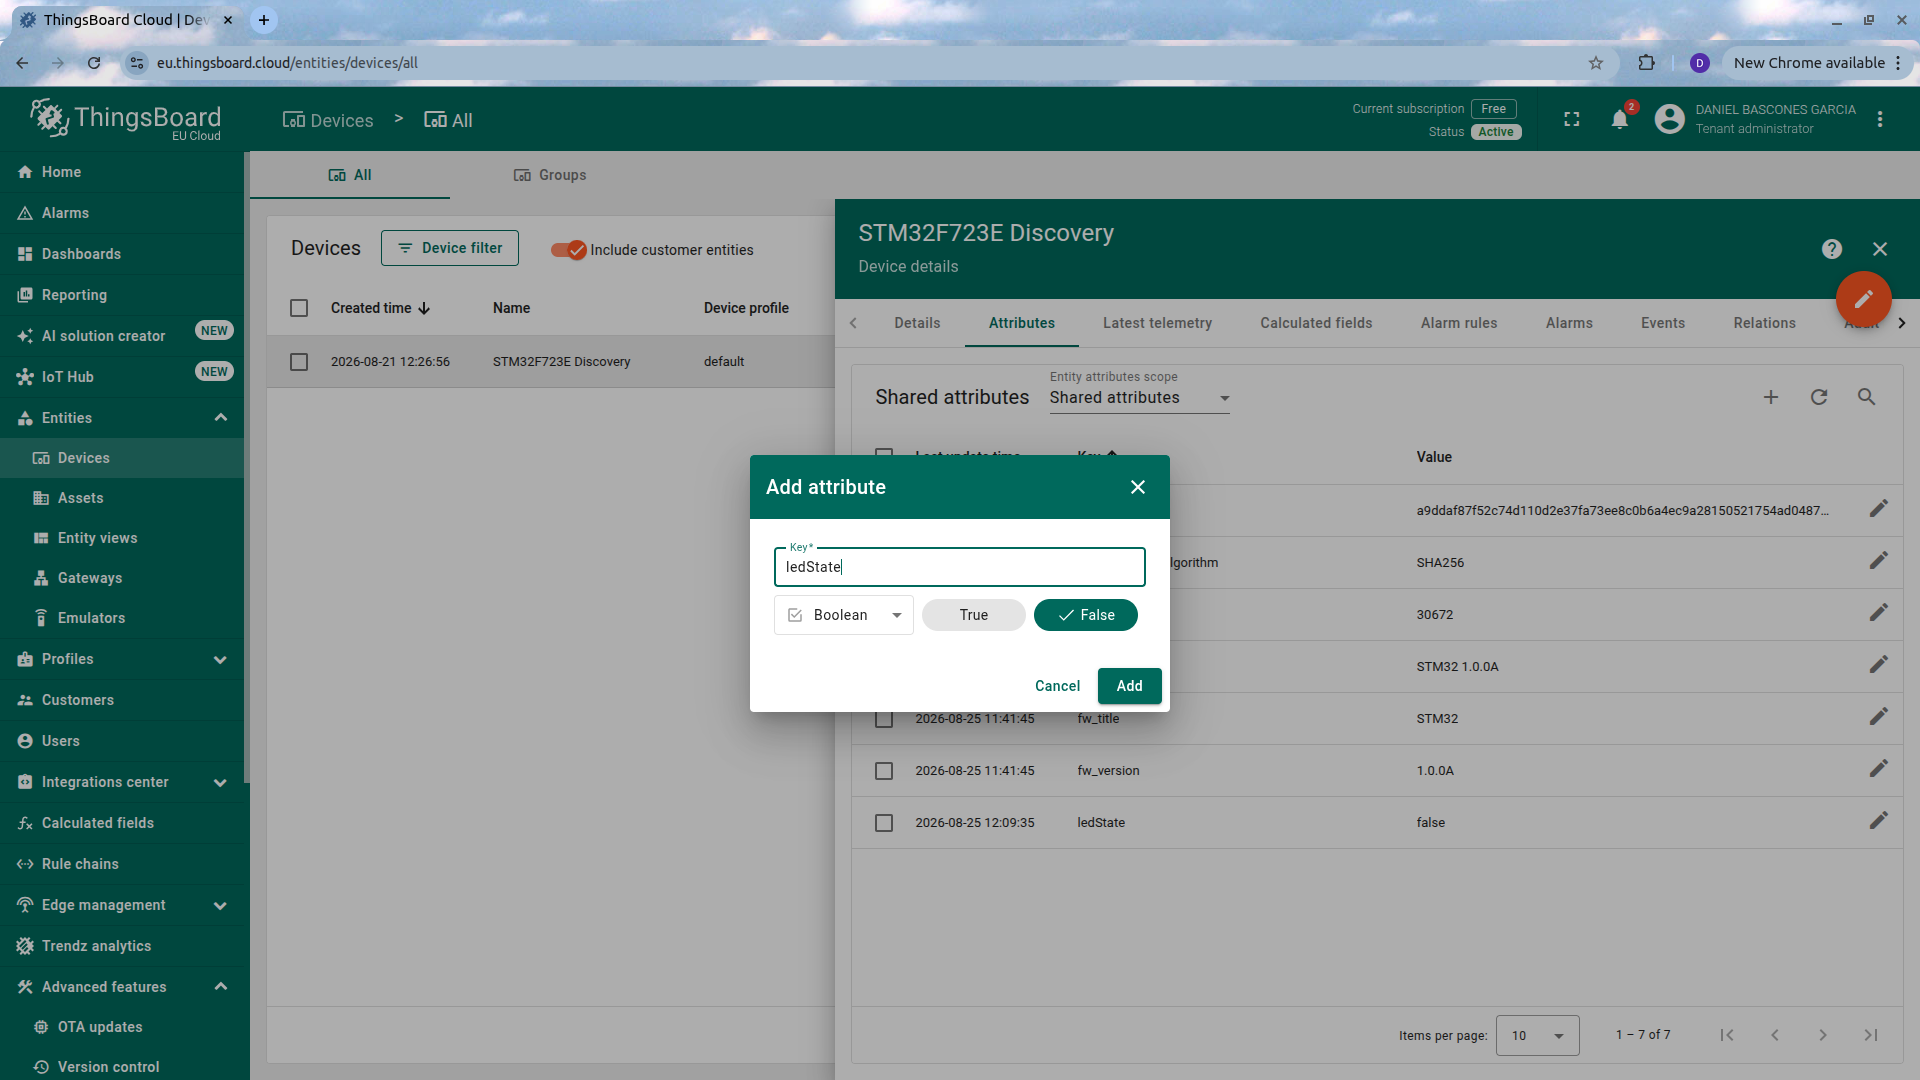
\includegraphics[width=\textwidth]{res/thingsboard_shared_attributes.png}
                \caption{Atributo compartido para nuestro dispositivo}
                \label{fig:thingsboard_shared_attributes}
            \end{figure}

            Ahora tenemos que añadir un botón que lo pueda gestionar. Añadimos a nuestro panel un widget ``single switch'', y lo configuramos como muestra la \Cref{fig:thingsboard_single_switch}. Básicamente lo que estamos haciendo es añadir un botón que cambiará este valor asociado a nuestro dispositivo.

            \begin{figure}
                \centering
                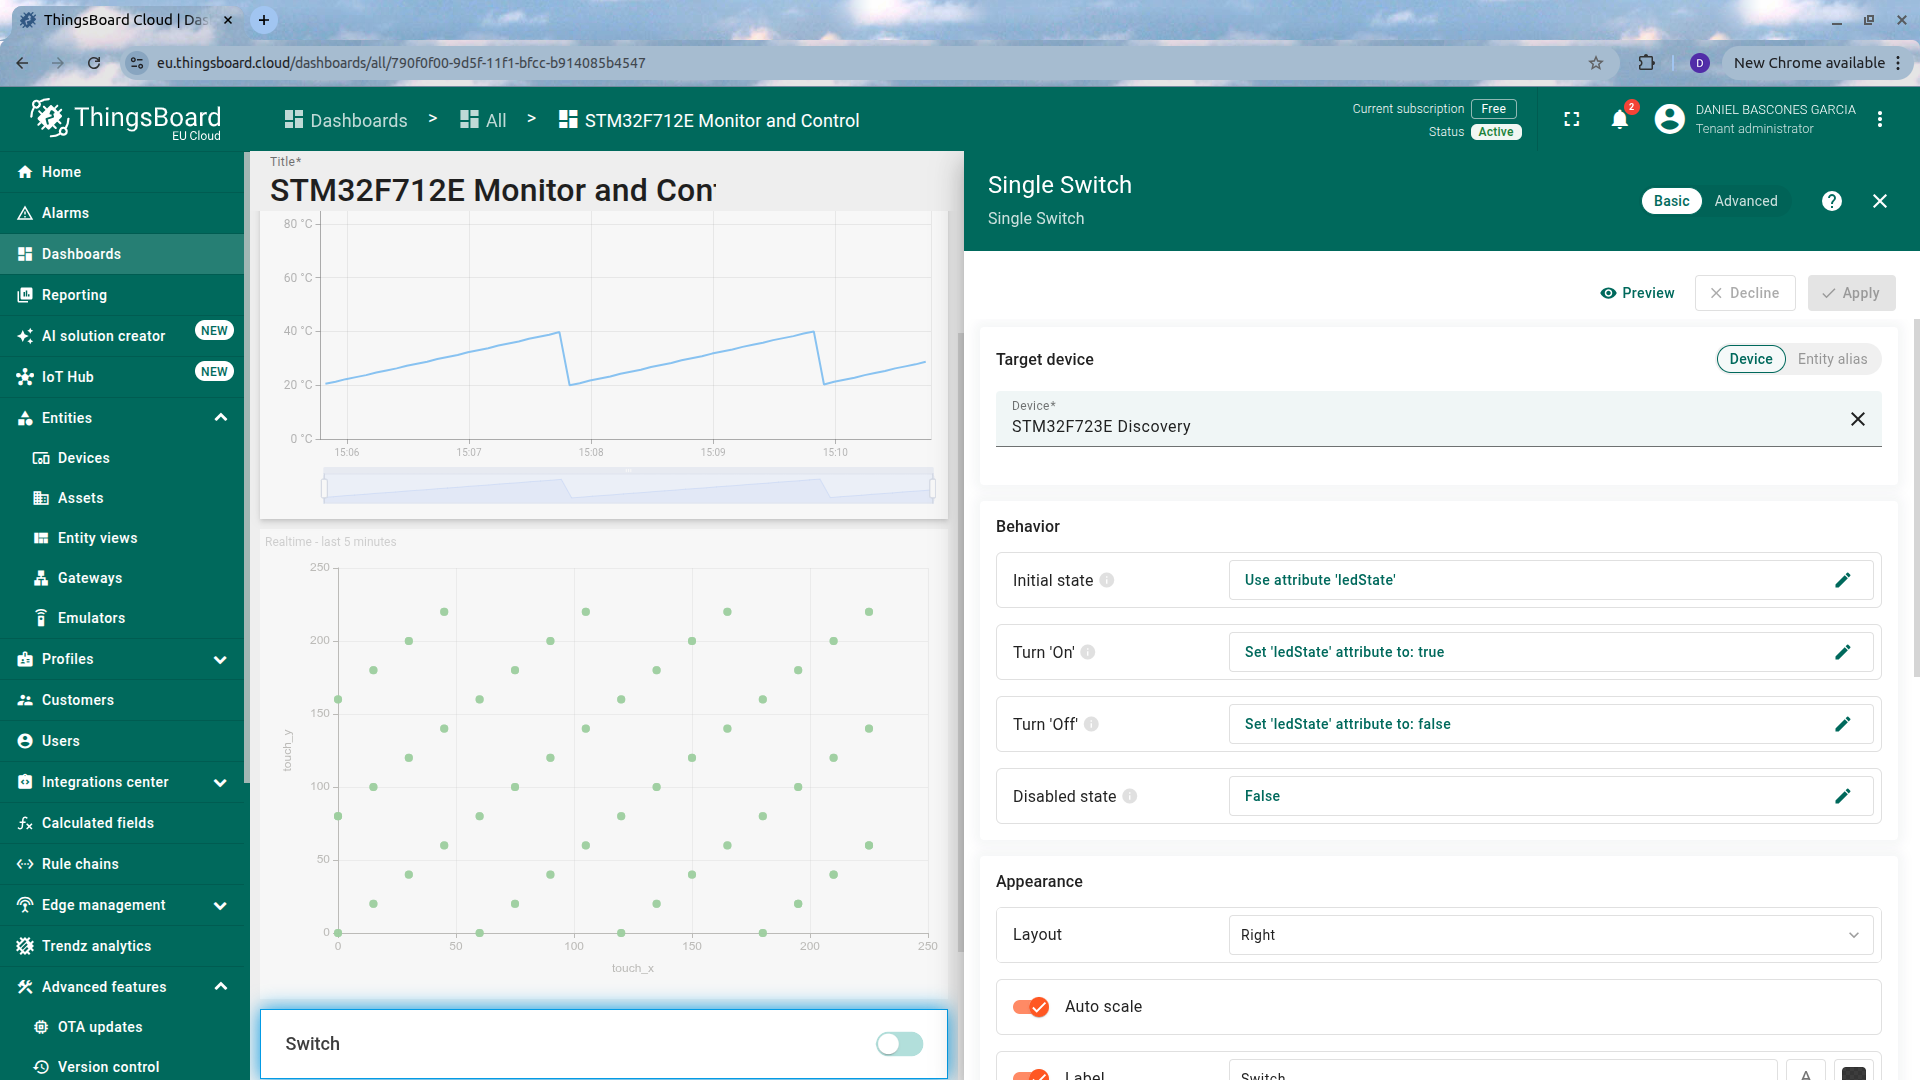
\includegraphics[width=\textwidth]{res/thingsboard_single_switch.png}
                \caption{Atributo compartido para nuestro dispositivo}
                \label{fig:thingsboard_single_switch}
            \end{figure}
            
            \emph{ThingsBoard}, como \emph{broker} que es, avisará al dispositivo cada vez que cambie este valor, ya que es un atributo compartido que debería actualizar. Si hacemos click, veremos que el LED ya cambia de color, pues la función de procesamiento de mensajes ya está hecha en la forma de \texttt{ESP01S\_ProcessMQTT}, que se llama repetidamente desde el bucle de \texttt{main.c}:

            Como es bastante larga, no la ponemos completa, pero consta de dos partes: en una primera, se extrae el paquete MQTT en crudo de la UART de entrada, y en una segunda, se parsea el paquete para extraer la información necesaria (básicamente, qué se ha actualizado):

            \begin{lstlisting}
                // Paho Deserializer
                unsigned char dup, retained;
                int qos, payloadlen;
                unsigned char* payload;
                MQTTString receivedTopic;

                if (MQTTDeserialize_publish(&dup, &qos, &retained, NULL, &receivedTopic,
                                            &payload, &payloadlen, packet, copy_len) == 1)
                {
                    Debug_Printf("[MQTT RX] %s\r\n", receivedTopic.lenstring.data);

                    char json_str[128] = {0};
                    uint16_t str_len = (payloadlen < sizeof(json_str) - 1) ? payloadlen : sizeof(json_str) - 1;
                    memcpy(json_str, payload, str_len);

                    // LED command processing
                    if (strstr(json_str, "\"ledState\":true"))        GPIO_PIN_WRITE(GPIOA, 7, GPIO_STATE_ONE);
                    else if (strstr(json_str, "\"ledState\":false"))   GPIO_PIN_WRITE(GPIOA, 7, GPIO_STATE_ZERO);

                }
            \end{lstlisting}

            Como se puede observar, si se recibe un mensaje conteniendo la cadena \texttt{"ledState":true} o \texttt{"ledState":false}, el LED cambiará su valor al recibido.

            \textbf{NOTA:} En realidad, la forma canónica de hacer esto es utilizando la clase \texttt{MQTTClient} y registrando \emph{callbacks} para atributos concretos recibidas, que llamarán a funciones que hagan la funcionalidad (valga la redundancia) asociada a dichos atributos. Sin embargo, la librería completa da algunos problemas de stack overflow. Si alguien se anima a optimizar esta práctica para que funcione (de manera consistente) con esa clase, es un buen proyecto final.


    \subsection{Para hacer más}

        Ahora que ya tienes la placa conectada con un servidor remoto, y puedes mandar datos y recibir comandos desde ella, puedes explorar las opciones de \emph{ThingsBoard} en general o de los \emph{dashboard} más concretamente, o hacer por ejemplo que los datos que se envían sean reales, en lugar de sintéticos. 

\end{document}